\documentclass[a4paper,12pt]{article}
\usepackage{graphicx} % For including images
\usepackage{amsmath}
\usepackage{geometry} % To adjust margins
\usepackage{tikz}
\usepackage{xcolor}
\usepackage{mathptmx} % Times New Roman-like font for pdflatex
\usepackage{helvet}   % Helvetica for sans-serif
\usepackage{courier}  % Courier for monospace
\usetikzlibrary{shapes}
\usetikzlibrary{positioning}
\geometry{top=1.5in, bottom=1.5in, left=1.2in, right=1.2in}

\definecolor{McGill Red}{HTML}{ED1B2F}
\definecolor{Solid Black}{HTML}{000000}
\definecolor{White}{HTML}{FFFFFF}
\definecolor{Pale Gray}{HTML}{F4F4F4}
\definecolor{Medium Gray}{HTML}{D4D4D4}

% Define custom colors
\definecolor{myblue}{HTML}{0072B2}
\definecolor{myorange}{HTML}{E69F00}
\definecolor{mygreen}{HTML}{009E73}
\definecolor{mypurple}{HTML}{CC79A7}

\begin{document}

% Cover Page
\begin{titlepage}
    \begin{center}
        
        % Title
        \textbf{\Huge COMP 307 Project}\\[1.5cm]
        \Large MyMcGillMeetings\\
        % Subtitle or Description (optional)
        \Large Design Report\\[2cm]
        
        % Author's Name
        \textbf{\Large Team Members:}\\
        \Large Gan, Jeffrey, 261054762\\
        \Large Renaudie, Lucas, 261045005\\
        \Large Rhodes, Danielle, 261002836\\
        \Large Tu, Ping-Chieh, 261098947\\
        \Large Wang, Melody, 261053910\\[1.5cm]
        
        % Additional Details
        \textbf{\Large Submission Date:}\\
        \Large 2024 November 25$^{\text{th}}$ \\[2cm]
        
        % Institution and Date
        \textbf{\Large McGill University}\\
        \Large Faculty of Science\\[1cm]
    \end{center}
\end{titlepage}
% End of Cover Page

\section*{Branding}
\subsection*{Title}
MyMcGillMeetings
\subsection*{Colour palette}
We decide to follow the McGill style of colour.\\
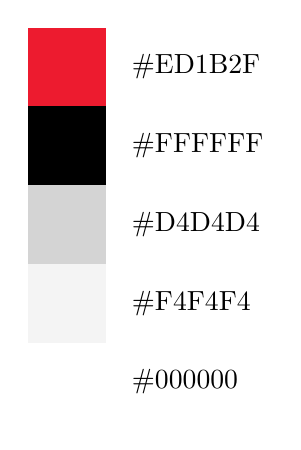
\begin{tikzpicture}
    % Draw a grid of color swatches with labels
    \foreach \colorname/\colordef [count=\i from 0] in {
        McGill Red/ED1B2F,
        Solid Black/FFFFFF,
        Medium Gray/D4D4D4,
        Pale Gray/F4F4F4,
        White/000000
    } {
        % Color square
        \fill[\colorname] (0, -\i) rectangle (1, -\i-1);
        % Color name
        \node[anchor=west] at (1.2, -\i-0.5) {\#\colordef};
    }
\end{tikzpicture}\\
We will also use different opacity/shade of the above color palette.
\subsection*{Typefaces}
We will use Arial for all of the content.
\subsection*{Logo}

\includegraphics[scale=0.1]{Logo.png}
\newpage
\section*{Storyboard}
Below is our storyboard for our website. Rectangles are for webpages, ellipses are for programs, and cylinders are for databases. Member DB and User DB are repeating twice but they are refer to the same database each. Red rectangle pages are only visible to members.
\begin{center}
    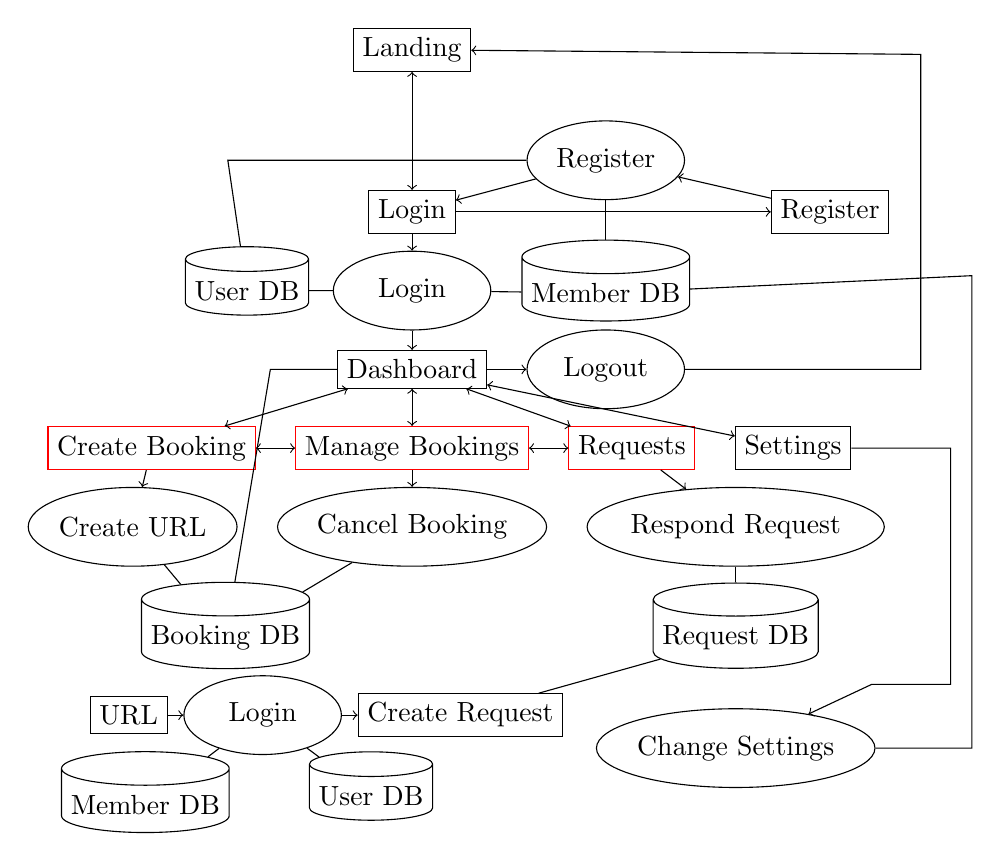
\begin{tikzpicture}[prog/.style={draw,ellipse,minimum width=2cm, minimum height=1cm, inner sep=0pt}, page/.style={draw, rectangle}, pagemem/.style={draw=red,rectangle}, db/.style={
        shape=cylinder,
        shape border rotate=90,
        draw,
        aspect = 0.2}]
        \node[page] (Dash) {Dashboard};
        \node[prog] (Log) [above of=Dash] {Login};
        \node[page] (Login) [above of=Log] {Login};

        \node[pagemem] (manage) [below of=Dash] {Manage Bookings};
        \node[pagemem] (create) [left=5mm of manage] {Create Booking};
        \node[pagemem] (request) [right=5mm of manage] {Requests};
        
        \node[prog] (cancel) [below of=manage] {Cancel Booking};
        \node[prog] (createBooking) [left=5mm of cancel] {Create URL};
        \node[prog] (respond) [right=5mm of cancel] {Respond Request};
        
        \node[db] (reqDB) [below=2mm of respond] {Request DB};
        \node[db] (bookDB) [left=43.5mm of reqDB] {Booking DB};
        

        \node[prog] (out) [right=5mm of Dash] {Logout};
        \node[page] (Reg) [right=40mm of Login] {Register};
        \node[db] (mem) [above=1mm of out] {Member DB};
        \node[db] (UserDB) [left=3mm of Log] {User DB};

        \node[page] (set) [right=5mm of request] {Settings};
        \node[prog] (changset) [below=5mm of reqDB] {Change Settings};
        
        \node[prog] (reg) [above=5mm of mem] {Register};

        \node[page] (Landing) [above=15mm of Login] {Landing};


        \node[page] (url) [below left=5mm of bookDB] {URL};
        \node[prog] (urllog) [right=2mm of url] {Login};
        \node[page] (req) [right=2mm of urllog] {Create Request};

        \node[db] (userdb) [below right=2mm of urllog] {User DB};
        \node[db] (memdb) [below left=2mm of urllog] {Member DB};

        \draw[->] (Log) -- (Dash);
        \draw[->] (Login) -- (Log);
        \draw[<->] (Dash) -- (manage);
        \draw[<->] (Dash) -- (create);
        \draw[<->] (Dash) -- (request);
        \draw[<->] (manage) -- (request);
        \draw[<->] (manage) -- (create);
        \draw[->] (manage) -- (cancel);
        \draw[->] (request) -- (respond);
        \draw[->] (create) -- (createBooking);
        \draw[-] (respond) -- (reqDB);
        \draw[-] (createBooking) -- (bookDB);
        \draw[-] (cancel) -- (bookDB);
        \draw[-] (req) -- (reqDB);
        \draw[-] (Log) -- (mem);
        \draw[-] (Log) -- (UserDB);
        \draw[->] (Login) -- (Reg);
        \draw[->] (Reg) -- (reg);
        \draw[->] (reg) -- (Login);
        \draw[<->] (Landing) -- (Login);
        \draw[->] (Dash) -- (out);
        \draw[->] (out) -- ++(4, 0) % Move left
                 -- ++(0, 4)    % Move up
                 -- (Landing);  % Move right to the target
        \draw[<->] (set) -- (Dash);
        \draw[->] (set) -- ++ (2,0)
                    -- ++ (0,-3)
                    -- ++ (-1, 0)
                    -- (changset);
        \draw[-] (changset) -- ++ (3,0)
                    -- ++ (0,6)
                    -- (mem);
        \draw[-] (reg) -- (mem);
        \draw[-] (Dash) -- ++ (-1.8,0)
        
                    -- (bookDB);
        \draw[->] (url) -- (urllog);
        \draw[->] (urllog) -- (req);
        \draw[-] (urllog) -- (userdb);
        \draw[-] (urllog) -- (memdb);
        \draw[-] (reg) -- ++ (-4.8,0)
                    -- (UserDB);
    \end{tikzpicture}
\end{center}
Public pages: Landing, Login, Register, URL\\
Private pages: Dashboard, Create Booking, Manage Booking, Requests, Settings, Create Request\\
List of features for all users:
\begin{itemize}
    \item Dashboard: Sees previous/upcoming appointments + change/cancel appointments.
    \item Create Request: Request a meeting upon URL.
    \item Settings: Change user settings.
\end{itemize}
List of features for McGill members:
\begin{itemize}
    \item Manage Bookings: Modify existing bookings.
    \item Create Bookings: Create a new booking.
    \item Requests: See incoming request for bookings.
\end{itemize}
\newpage
\section*{Screen mock-up}
\subsection*{Landing}
\begin{tikzpicture}
    \node[draw=black, thick, inner sep=0] {
\includegraphics[scale=0.2]{landing.png}};
\end{tikzpicture}
\subsection*{Login/Register}
Users are able to choose between whether they are a McGill member or not.\\
\begin{tikzpicture}
    \node[draw=black, thick, inner sep=0] {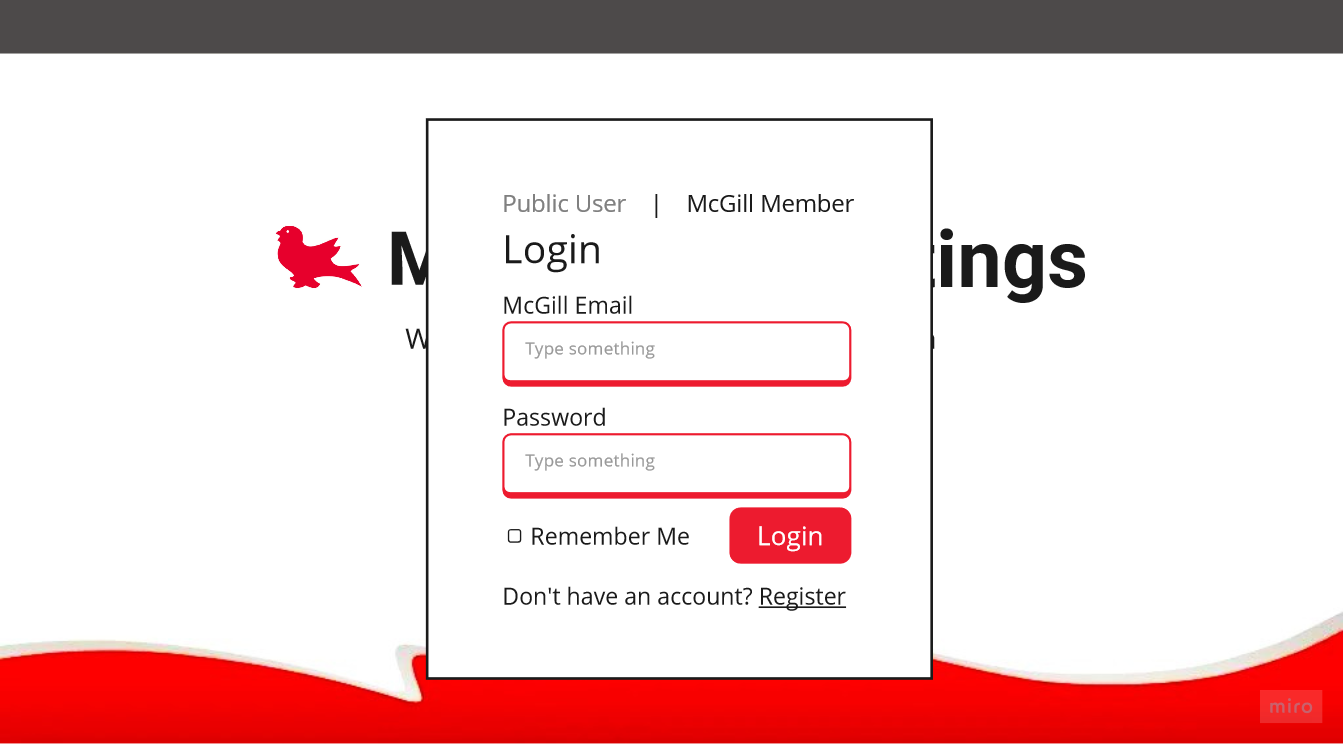
\includegraphics[scale=0.2]{Login.png}};
\end{tikzpicture}\\
\begin{tikzpicture}
    \node[draw=black, thick, inner sep=0] {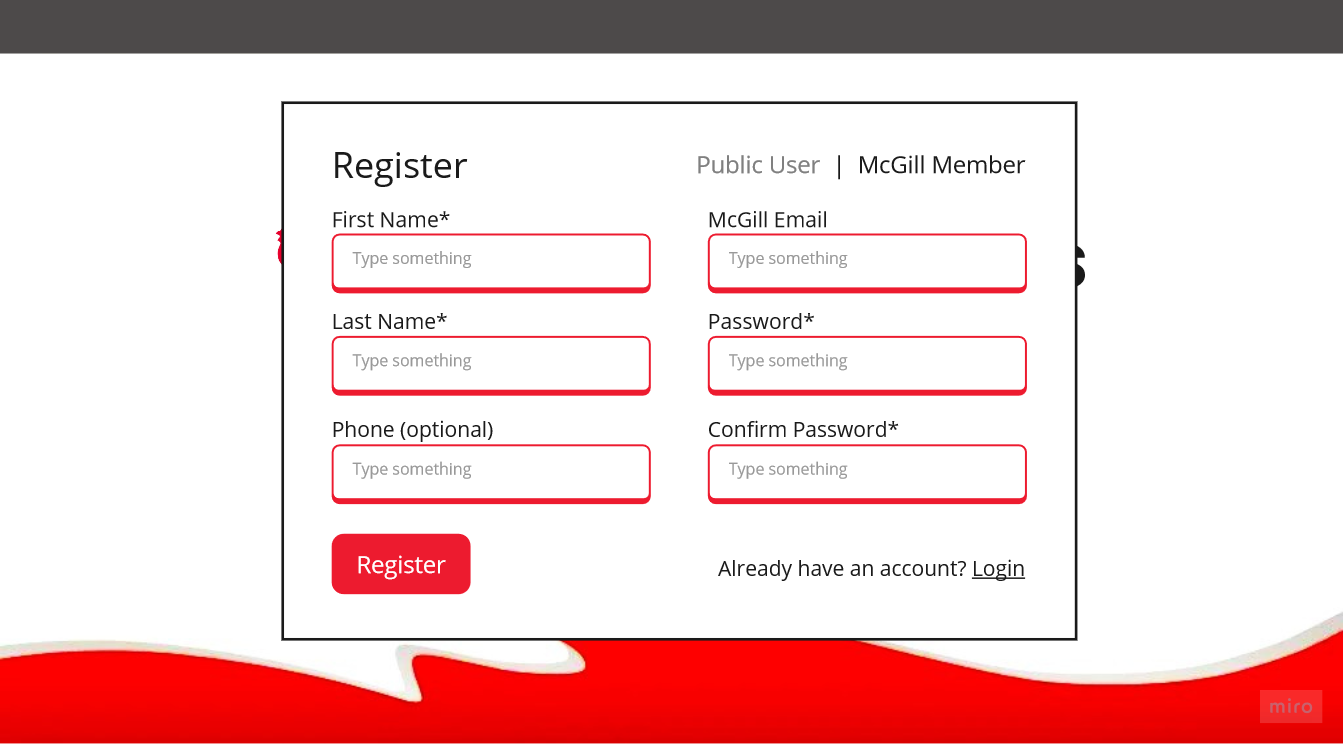
\includegraphics[scale=0.2]{Register.png}};
\end{tikzpicture}
\subsection*{Dashboard}
For McGill members:\\
\begin{tikzpicture}
    \node[draw=black, thick, inner sep=0] {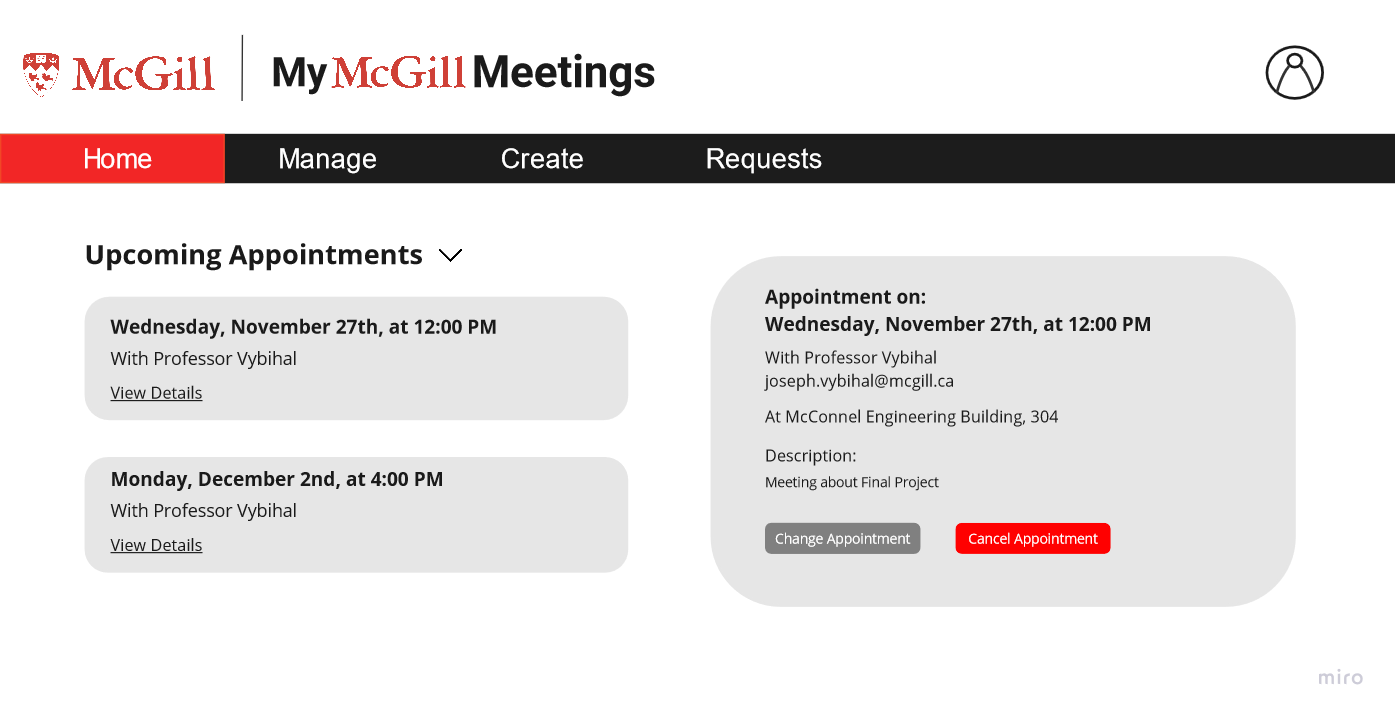
\includegraphics[scale=0.2]{Home1.png}};
\end{tikzpicture}\\
\begin{tikzpicture}
    \node[draw=black, thick, inner sep=0] {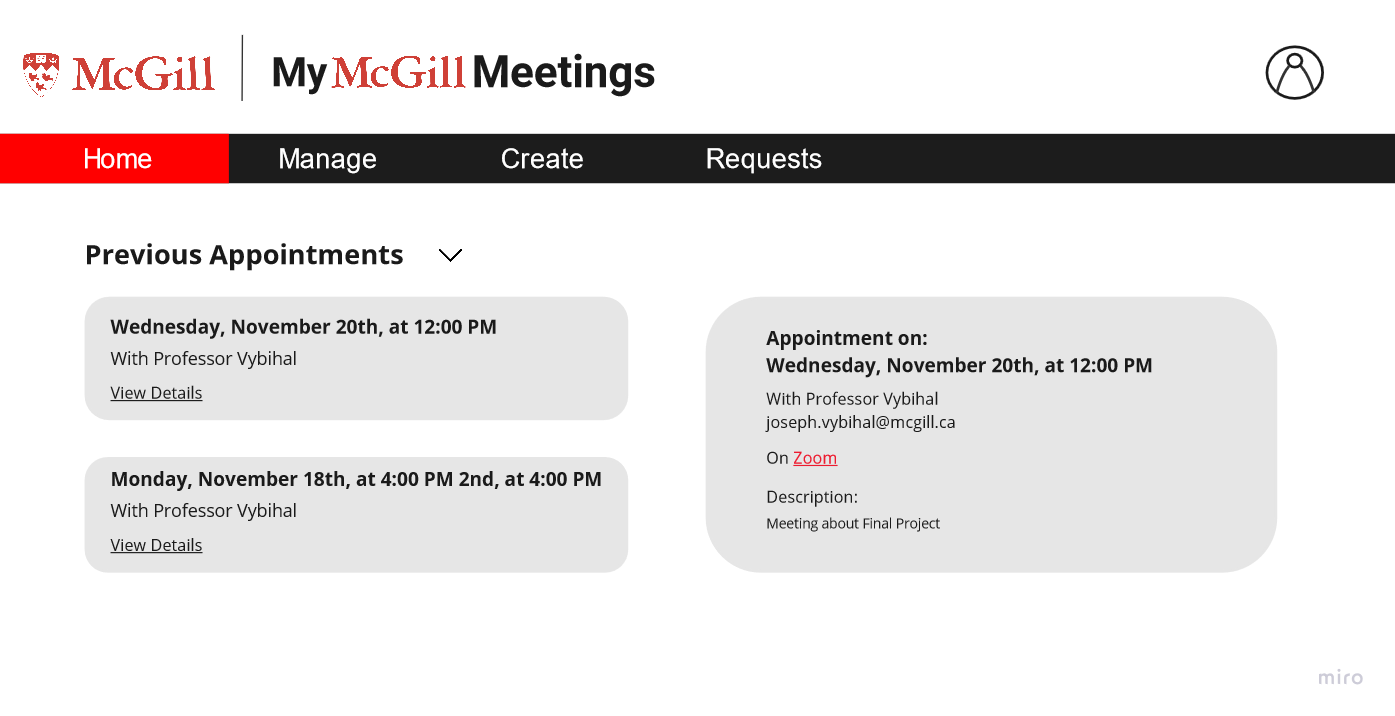
\includegraphics[scale=0.2]{Home2.png}};
\end{tikzpicture}\\
For non McGill member example:\\
\begin{tikzpicture}
    \node[draw=black, thick, inner sep=0] {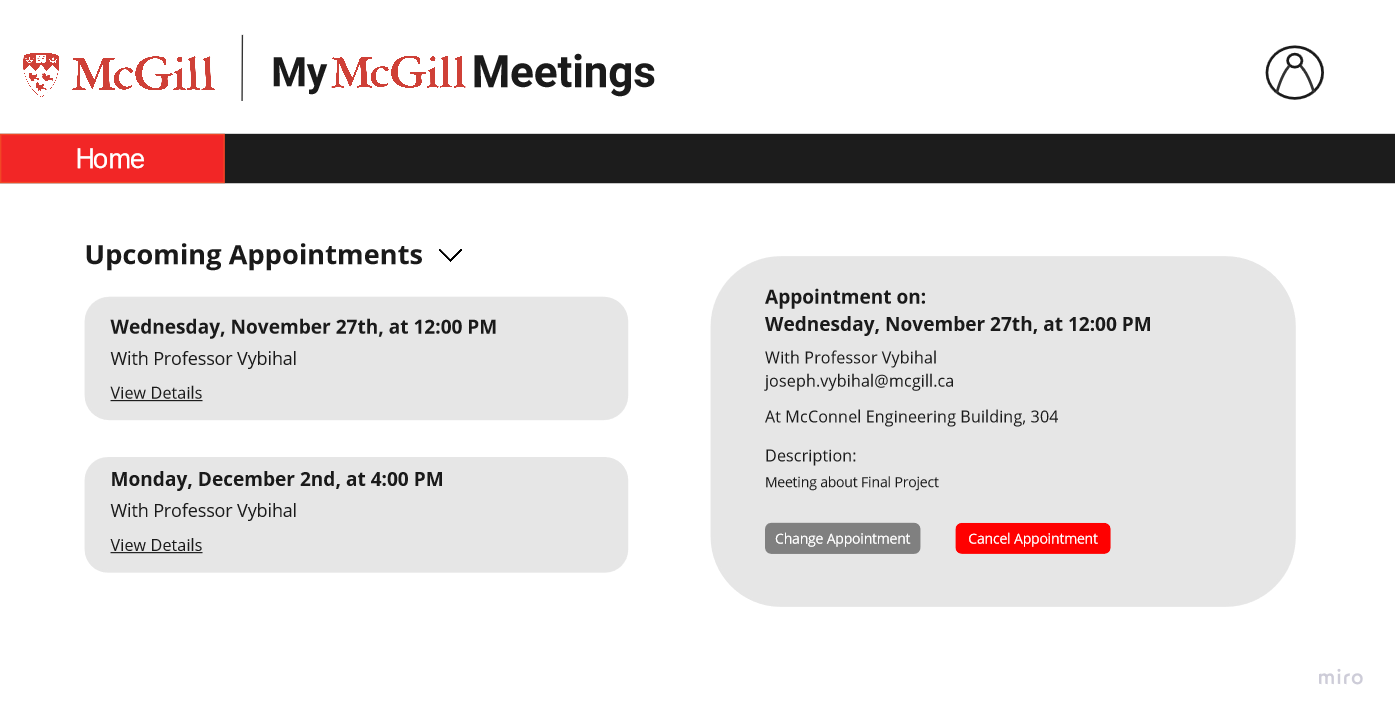
\includegraphics[scale=0.2]{Home3.png}};
\end{tikzpicture}\\
The navigation bar for non McGill member is different from McGill members. We will only show screen mock-ups for McGill members below.
\subsection*{URL}
\begin{tikzpicture}
    \node[draw=black, thick, inner sep=0] {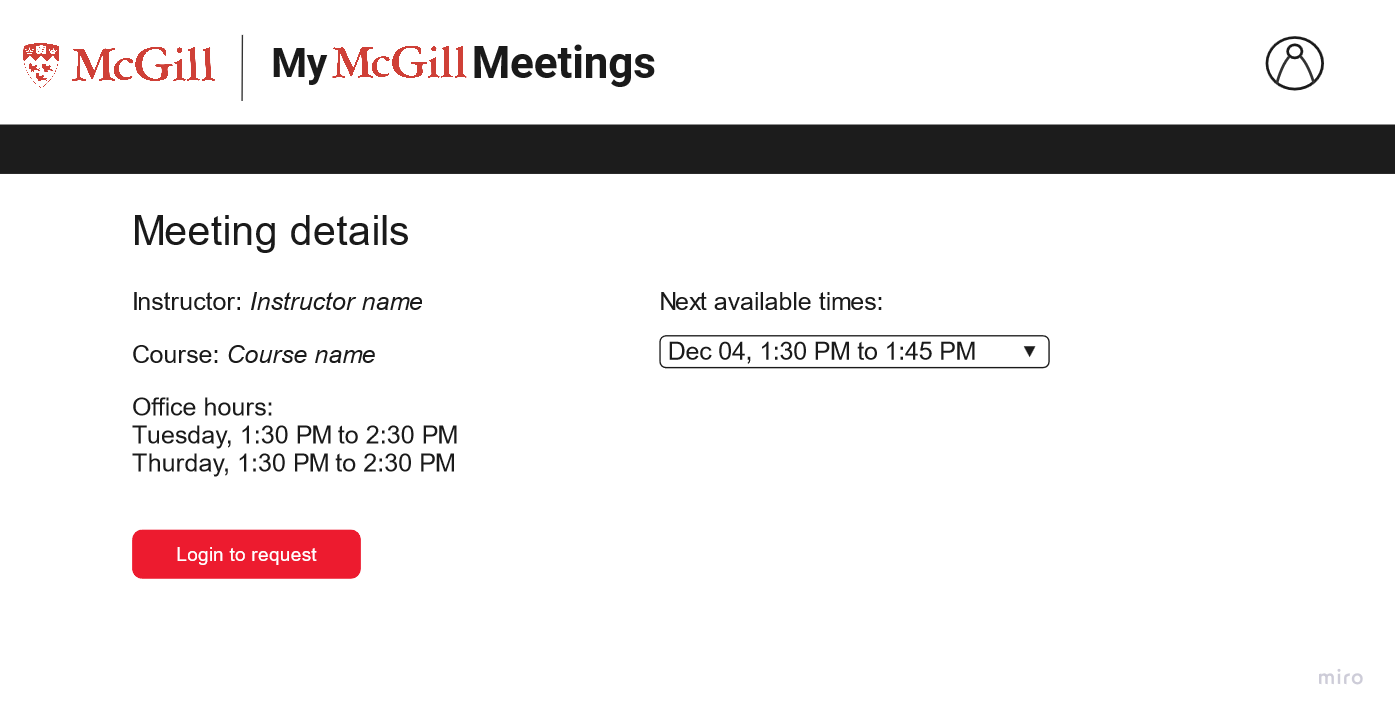
\includegraphics[scale=0.2]{url.png}};
\end{tikzpicture}\\
After Logging in, it will take the user to request meeting page
\subsection*{Request Meeting}
\begin{tikzpicture}
    \node[draw=black, thick, inner sep=0] {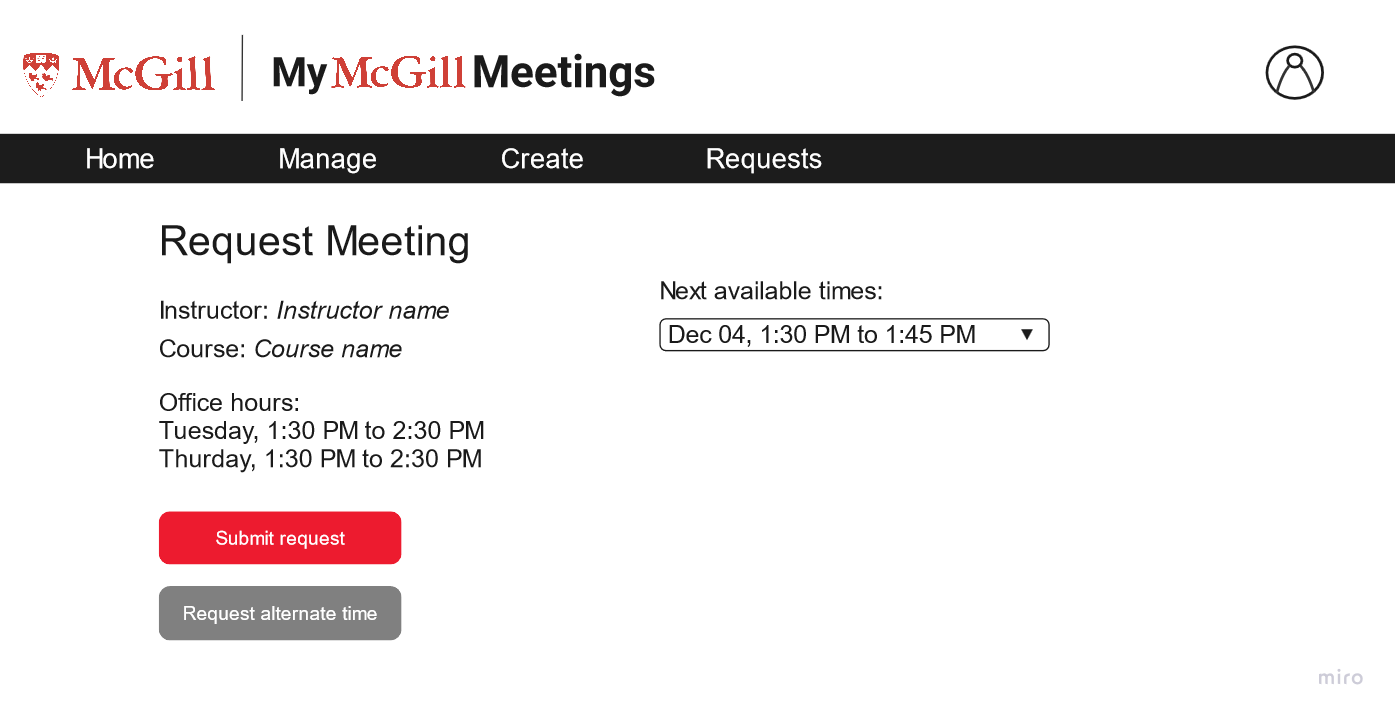
\includegraphics[scale=0.2]{requestMeeting.png}};
\end{tikzpicture}
\subsection*{Request alternate meeting time}
\begin{tikzpicture}
    \node[draw=black, thick, inner sep=0] {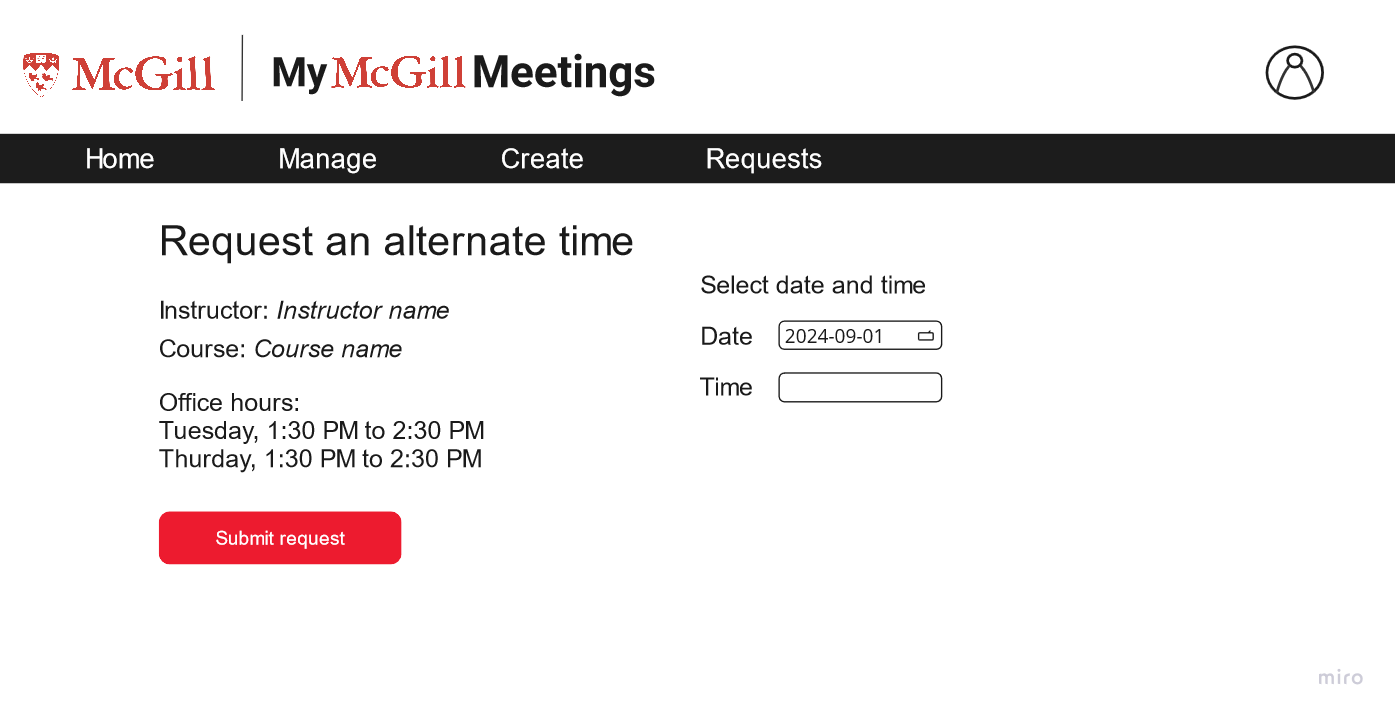
\includegraphics[scale=0.2]{alternate.png}};
\end{tikzpicture}
\subsection*{Create Booking}
\begin{tikzpicture}
    \node[draw=black, thick, inner sep=0] {\includegraphics[scale=0.2]{createbook.png}};
\end{tikzpicture}\\
\begin{tikzpicture}
    \node[draw=black, thick, inner sep=0] {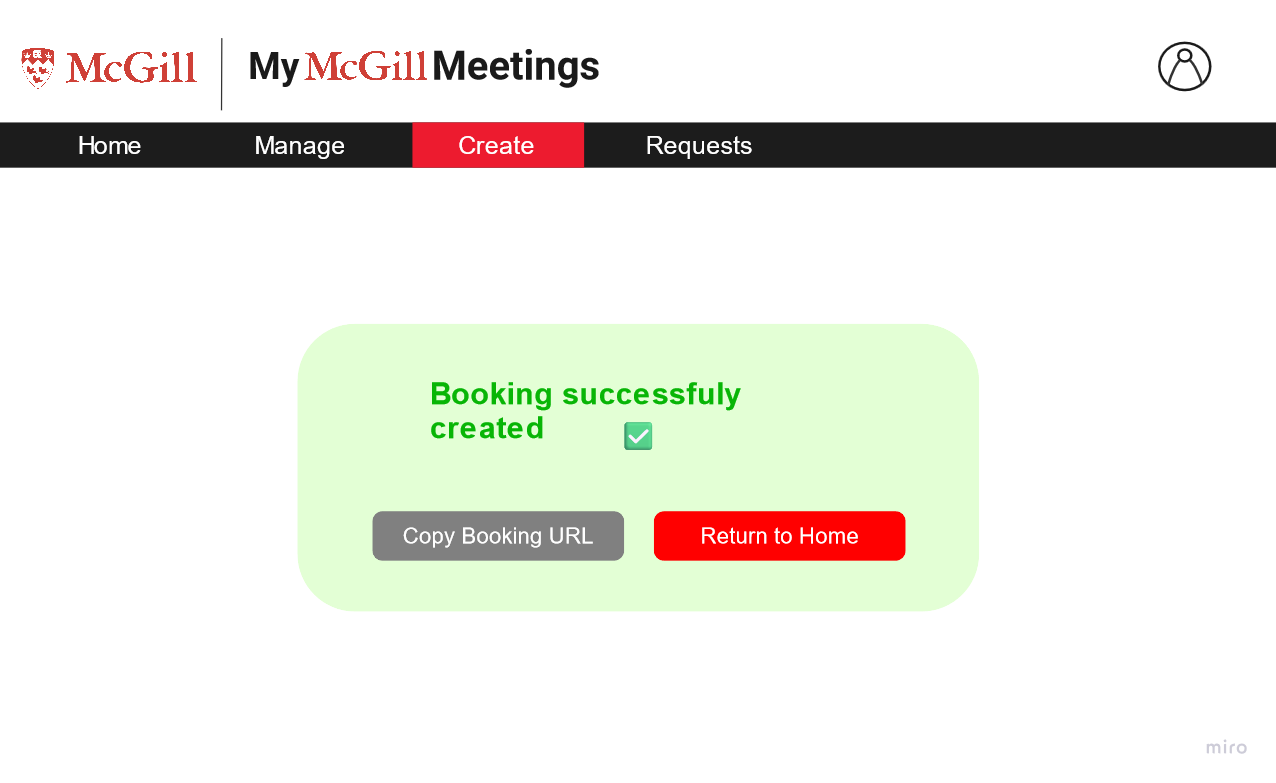
\includegraphics[scale=0.2]{success.png}};
\end{tikzpicture}
\end{document}